\documentclass[10pt]{article}
\setlength{\parskip}{0.25\baselineskip}
\usepackage[margin=1in]{geometry} 
\usepackage{amsmath,amsthm,amssymb, graphicx, multicol, array}
\usepackage[font=small,labelfont=bf]{caption}
\usepackage{float}

\newcommand{\supp}{{\text{supp}}} 
\newcommand{\bv}{{\text{BV}}}
\newcommand{\ac}{{\text{AC}}}

\newenvironment{problem}[2][]{\begin{trivlist}
\item[\hskip \labelsep {\bfseries #1}\hskip \labelsep {\bfseries #2.}]}{\end{trivlist}}

\begin{document}
 
\title{Homework \#5}
\author{Eric Tao\\
Math 123: Homework \#5}
\maketitle

\begin{problem}{Question 1}

Let $\{ x_i \}_{i=1}^n \subset \mathbb{R}^D$ be a discrete set on unique points. Recall that the DBSCAN algorithm depends on two parameters: $\epsilon$ and MinPts.

(a) Describe the behavior of DBSCAN as $\epsilon \to \infty$ and $\epsilon \to 0^+$.

(b) Describe the behavior of DBSCAN as MinPts $\to \infty$ and as MinPts $\to 0^+$.

\end{problem}

\begin{proof}[Solution]

(a)

We recall that $\epsilon$ represents the distance under which a point is considered "close enough". Fix some $1 < $ MinPts $ \leq n$ (for sanity, as of course if MinPts $\leq 1$, then everything is automatically a core point, due to itself being within $\epsilon$ automatically, and if MinPts $\geq n+1$, every point is automatically an outlier, as there are only $n$ total points), and fix some data point $x_i$. Since there are a finite number of points $n$, we may look at the set $\{ \Vert x_j - x_i \Vert : 1 \leq j \leq n \}$. This is a set of real numbers, finite. Therefore, it achieves a maximum, call that value $M_{x_i}$. Consider any $\epsilon > M_{x_i}$. For such an $\epsilon$ and for any other point $x_j$, we have that:

$$ \Vert x_j - x_i \Vert \leq M_{x_i}  < \epsilon $$

Thus, so long as MinPts is a reasonable parameter for our set, that is, no larger than the size of the set, we have that every point is within $\epsilon$ of $x_i$, and thus $x_i$ is a core point as $\epsilon \to \infty$. In particular, we may choose $\epsilon$ as it grows to $\infty$ to be larger than all such $M_{x_i}$, since across the index $i$, this too is a finite set of real numbers, which achives a maximum. Thus, repeating this argument for any arbitrary point $x_i$, DBSCAN will indicate that every point is a core point of a single cluster as $\epsilon \to \infty$.

Conversely, suppose $\epsilon \to 0$. In a similar fashion then, we fix a MinPts, $x_i$, and consider the set $\{ \Vert x_i - x_j \Vert : i \not = j \}$. Because we have that the data points are unique, this must be a set of non-negative numbers, finite. Thus, the set achieves a minimum, call this $m_{x_i}$. If we choose an $0 < \epsilon < m_{x_i}$, then we have that, for any other point $x_j$:

$$  \Vert x_j - x_i \Vert \geq m_{x_i}  > \epsilon$$

and thus, $x_i$ is an outlier point. Again, since the set of $m_{x_i}$ is a finite set of non-negative real numbers, this too attains a minimum. We then can choose $\epsilon$ to be greater than 0, but less than every $m_{x_i}$ and repeat the argument to say that DBSCAN will indicate that every point is an outlier as $\epsilon \to 0^+$.

(b)

In a similar fashion, we may look at MinPts, while keeping $\epsilon$ fixed. Clearly, if MinPts is larger than $n$, the number of data points in a set, every point must be an outlier, since the set of points within $\epsilon$ can only be as large as the underlying data set. 

The reverse is clear as well, as regardless of the $\epsilon \geq 0$, when MinPts is equal to 1, every point $x_i$ is a core point, since $x_i$ is a point within $0 \leq \epsilon$ distance from $x_i$. However, we do note the edge case for if $\epsilon < 0$, then because distance functions are non-negative, every point remains an outlier regardless, unless MinPts is exactly equal to 0, as cardinalities of sets are non-negative.

\end{proof}

\begin{problem}{Question 2}

Let $L = D - W \in \mathbb{R}^{n \times n}$ be the graph Laplacian for data with an associated symmetric weight matrix $W$, and $w_{ij} \in [0,1]$ for all $i,j = 1,...,n$.

(a) Show $L$ is positive semidefinite.

(b) Show $L$ is not positive definite by proving $0$ is an eigenvalue of $L$.

\end{problem}

\begin{proof}[Solution]

(a)

Let $y \in \mathbb{R}^n$, realized as a column vector.

Consider the quantity $y^T L y$. Specifically, since $L = D - W$, we have that:

$$ (Ly)_i = (Dy)_i - (Wy)_i = \sum_{j=1}^n w_{ij} y_i - \sum_{j =1}^n w_{ij} y_j = \sum_{j=1}^n w_{ij} (y_i - y_j) $$

Thus, we have that:

$$ y^T Ly = \sum_{i=1}^n \sum_{j=1}^n  w_{ij} (y_i - y_j) y_i $$

Here, we look at a trick: Consider relabeling $i \to j, j \to i$ and then interchanging the summation. This does not change our sum, but we would have:

$$ y^T Ly = \sum_{j=1}^n \sum_{i=1}^n w_{ji} (y_j - y_i)y_j = - \sum_{i=1}^n \sum_{j=1}^n w_{ji} (y_i - y_j) y_j $$

Summing these two equations, and noticing that because $W$ is symmetric, we have that $w_{ij} = w_{ji}$:

$$2(y^T L y) = \sum_{i=1}^n \sum_{j=1}^n  w_{ij} (y_i - y_j) y_i -  \sum_{i=1}^n \sum_{j=1}^n w_{ji} (y_i - y_j) y_j =  \sum_{i=1}^n \sum_{j=1}^n w_{ij} (y_i - y_j)^2$$

which, of course, implies that:

$$y^TLy =  \frac{1}{2} \sum_{i=1}^n \sum_{j=1}^n w_{ij} (y_i - y_j)^2$$

Now, by hypothesis, $w_{ij} \geq 0$. And, since $y \in \mathbb{R}^n$, $(y_i - y_j)^2 \geq 0$. Thus, this is a (double) sum of non-negative numbers, and hence must be non-negative, that is, $y^T L y \geq 0$ 

(b)

We notice from our computation, that we arrived at

$$y^TLy =  \frac{1}{2} \sum_{i=1}^n \sum_{j=1}^n w_{ij} (y_i - y_j)^2$$

Thus, choose any $y$ such that $y = a(1,...,1)$. Then, for all $i,j$, we have that $y_i = y_j$, and thus $y^TLy = 0$. Equivalently, looking at $(Ly)_i$, we have:

$$ (Ly)_i =  \sum_{j=1}^n w_{ij} (y_i - y_j) = 0$$

for all $i$.

Thus, for this choice of $y$, we have that:

$$Ly = 0$$ and thus, $0$ is an eigenvalue, and thus $L$ is not positive definite.

\end{proof}

\begin{problem}{Question 3}

Compute the graph Laplacian with $W_{ij} = \exp(-\Vert x_i - x_j \Vert_2^2/ \sigma^2)$ on the image in Ncut\_Data.mat using a range of $\sigma$ values. For each of these $\sigma$, use the second eigenvector (the one with second smallest eigenvalue) to segment the image by thresholding at $0$. Discuss the results. Do they make sense, and how do the results depend on $\sigma$?

\end{problem}

\begin{proof}[Solution]

Here follows some charts with two clusters from Ncut, with clusters coloured differently:

\begin{figure}[H]
\centering
\begin{minipage}{.5\textwidth}
  \centering
  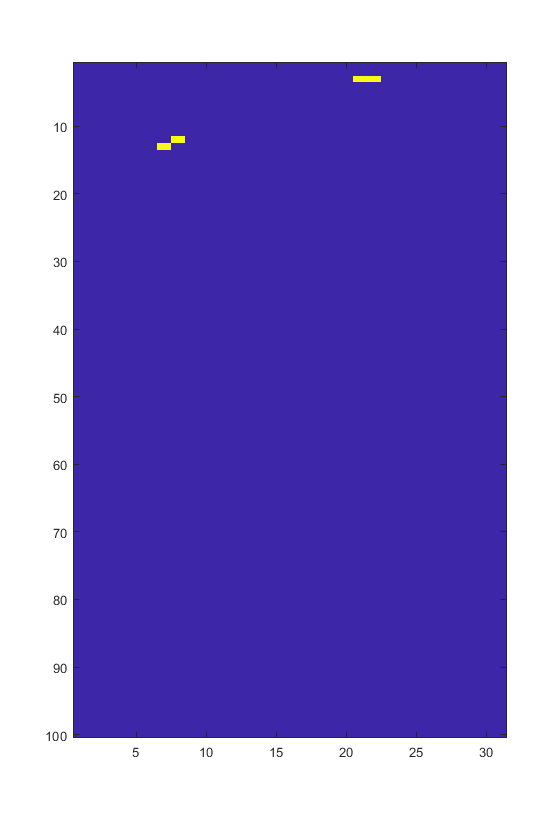
\includegraphics[width=\linewidth]{pepper_sigma_001}
  \captionof{figure}{$\sigma = 0.01$}
  \label{fig:test1}
\end{minipage}%
\begin{minipage}{.5\textwidth}
  \centering
  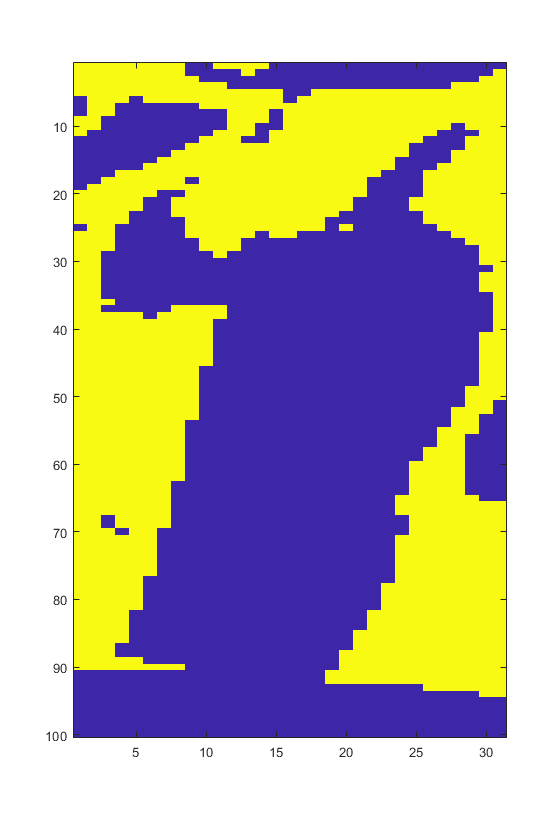
\includegraphics[width=\linewidth]{pepper_sigma_01}
  \captionof{figure}{$\sigma = 0.1$}
  \label{fig:test2}
\end{minipage}
\end{figure}

\begin{figure}[H]
\centering
\begin{minipage}{.5\textwidth}
  \centering
  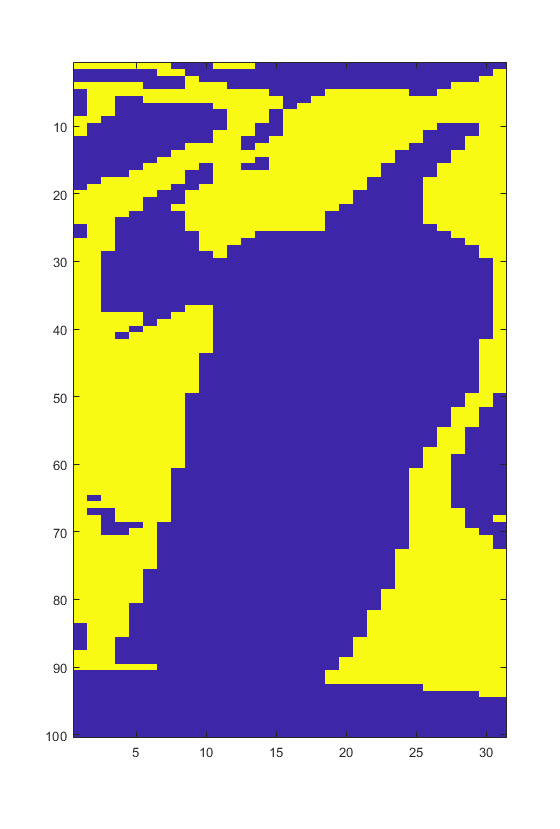
\includegraphics[width=\linewidth]{pepper_sigma_1}
  \captionof{figure}{$\sigma = 1$}
  \label{fig:test1}
\end{minipage}%
\begin{minipage}{.5\textwidth}
  \centering
  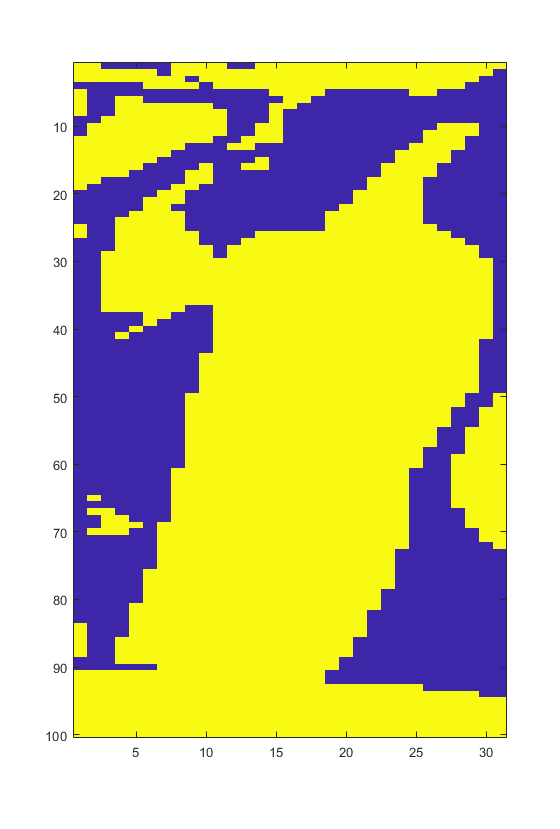
\includegraphics[width=\linewidth]{pepper_sigma_10}
  \captionof{figure}{$\sigma = 10$}
  \label{fig:test2}
\end{minipage}
\end{figure}

Generally speaking, these preserve the pepper strucure pretty well, in the sense that we do distinctly see a shadow of a figure in the main image for all but the first figure.

We notice that there is a sweet spot for $\sigma$ values that tries to make distinctions between the background and the pepper, but also have a sharp boundary. In the first figure, of course, $\sigma$ is too small to distinguish between background and foreground objects. On the other hand, as we increase $\sigma$ to 100, we notice that finer structures, especially those near the bottom left, become washed out a bit - we can see a gap that closes from figure 2, 3, and 4 that might be a gap between the pepper and its base, which may represent the background colors. In a nutshell, as $\sigma$ is very large or very small, we start to lose granularity in our clustering.

Lastly, we notice that clustering wise, as we increase $\sigma$, there is a switch from the pepper as being the blue color (i.e., below our threshold) to the yellow color (above the threshold). This isn't a very interesting thing actually, since it merely indicates which cluster has more points. 



\end{proof}



\end{document}